
\section{Chaînes de Markov}

\textbf{Introduction} Une chaîne de Markov est une suite de variables aléatoire (X$_n$,$n$ $\in N$) qui permet de modéliser l'évolution dynamique d’un système aléatoire : X$_n$ représente l’état du système à l’instant n. ("Nous pouvons considérer une chaine de markov comme une veriable aléatoire qui change avec le temps. Le temps discret n est alors un paramètre supplémentaire du système"). La propriété fondamentale des cahine des Markov, appelée propriété de Markov est que son évolution future ne dépend du passé qu'au travers de sa valeur actuelle : c'est à dire que X$_{n+1}$ ne dépend que de X$_n$ et non pas de  X$_{n-1}$,  X$_{n-2}$, .... Autrement dit, conditionnellement à  X$_{n}$, et $(X_0, ..., X_n)$ et $(X_{n+k}, k \in N)$ sont indépendants. Les applications des cahines de Markov sont très nombreuses (réseaux, simulation de propagation d'un virus (COVID), ingénérié financière, ...). Une chaine de Markov peut être associée à un graph orienté où le changement d'état s'effectue suivant une certain probabilité. \\

\noindent \textbf{Exemple:} Durant l’hiver Pierre peut être dans trois états: en bonne santé (état $x_1$), enrhumé (état $x_2$), grippé (état $x_3$). Son état le jour $n+1$ dépend de son état au jour $n$ et pas des jours précédents:
\begin{itemize}
    \item S’il est en bonne santé, il le reste le lendemain avec une probabilité égale à 5/6, il s’enrhume avec une probabilité égale à 1/12 et attrape la grippe avec une probabilité égale à 1/12;
    \item S’il est enrhumé il le reste avec une probabilité égale à 1/2, guérit avec une probabilité égale à 1/4 et attrape la grippe
avec une probabilité égale à 1/4;
    \item S’il est grippé, il le reste avec probabilité égale à 3/4 et guérit avec une probabilité égale à 1/4.
\end{itemize}

L’évolution de l’état de santé de Pierre peut être représenté par le graphe de la figure \ref{fig:graph_markov_exemple}.

\begin{figure}[h!]
    \centering
    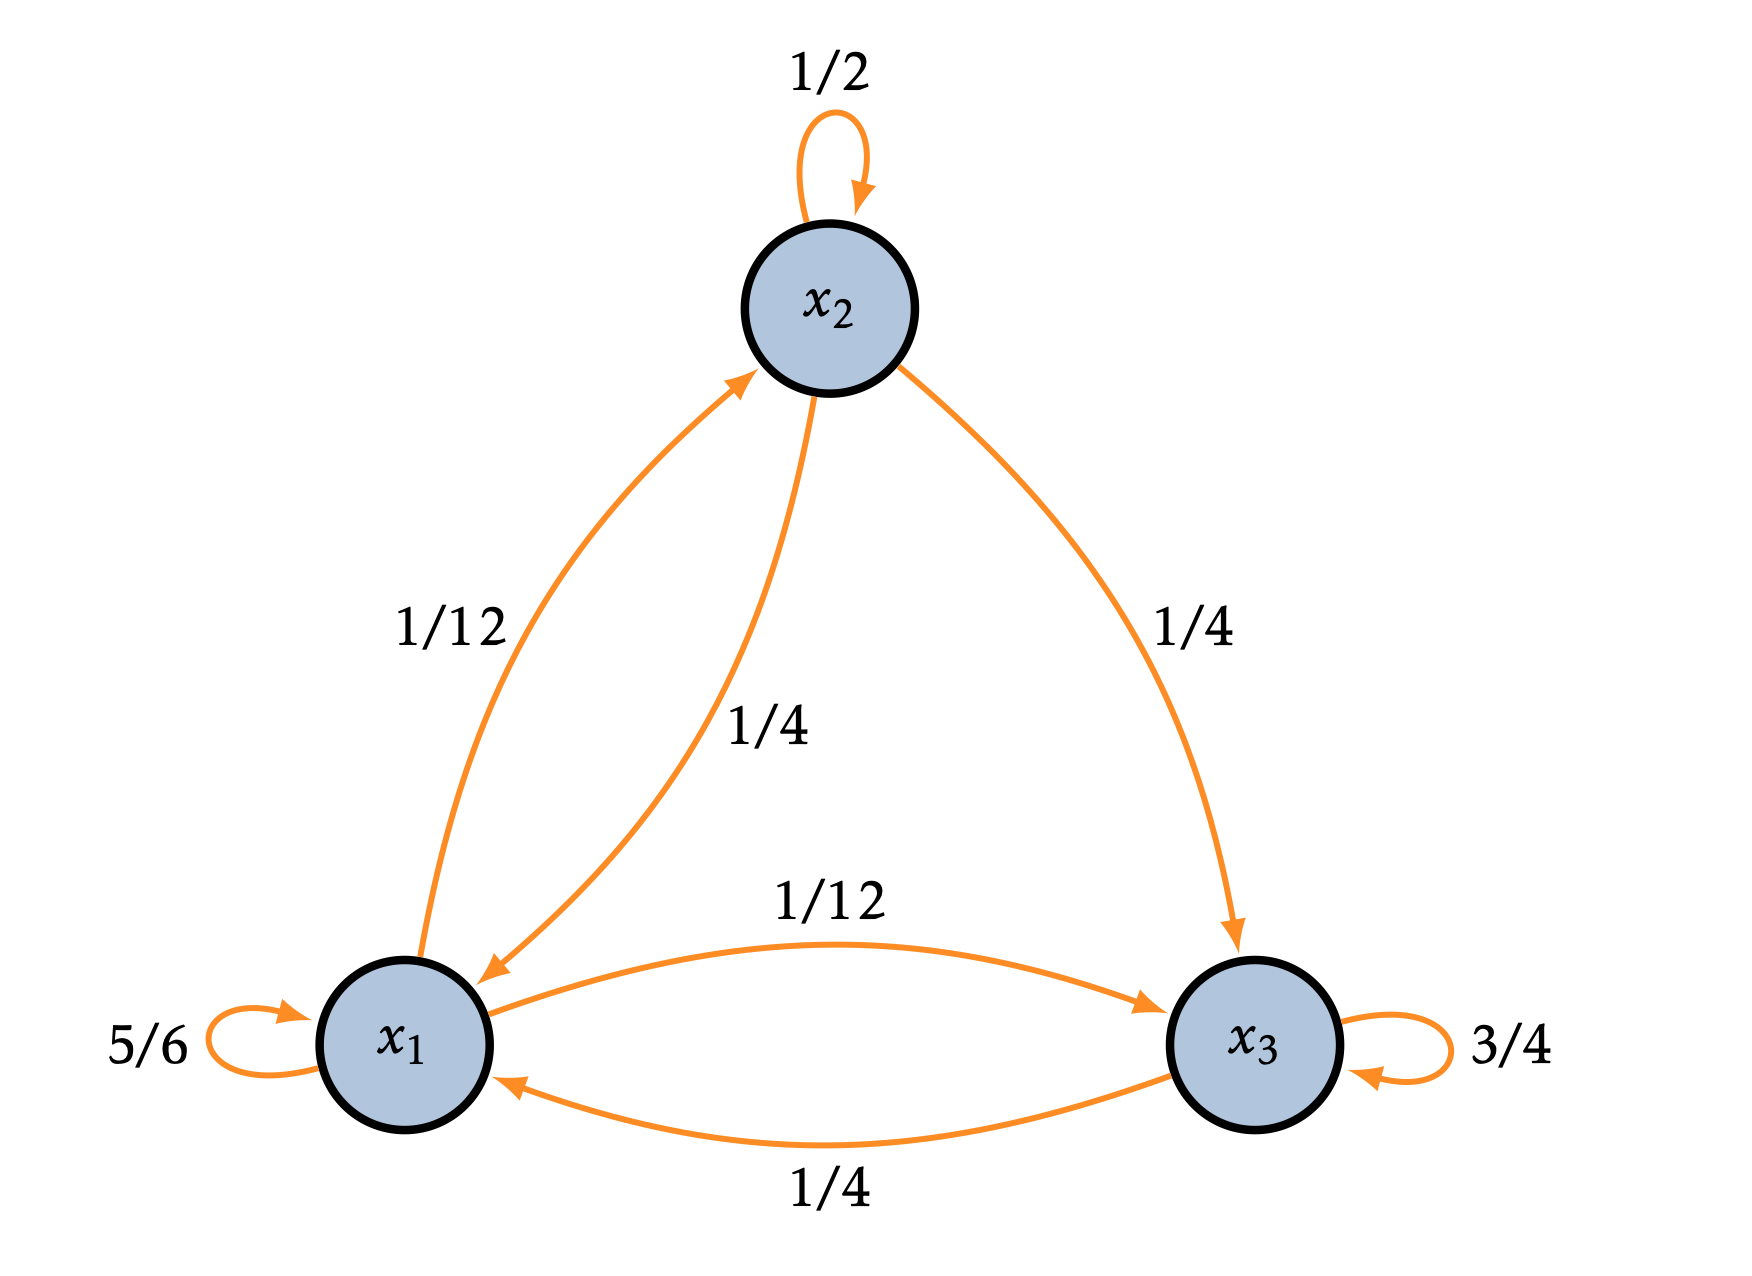
\includegraphics[width=.7\textwidth]{graph_markov_example.png}
    \caption{Exemple graph etat de santé de Pierre}
    \label{fig:graph_markov_exemple}
\end{figure}

La matrice $\mathbf{P}$ dont l'élément à l'indice $(i,j)$ (ligne $i$, colonne $j$) est $p_{ij}$ est appelée \textit{matrice de transition}. Si on a $N$ états, $P$ est de dimension $N \times N$ ($N$ lignes et $N$ colonnes). Si les chaînes sont homogènes, $\mathbf{P}$ \textbf{a deux propriétés importantes}: i, $p_{ij} \geq 0$ et ii, $\sum_i p_{ij} = 1$ (i.e chaque élément de la matrice est supérieur ou égal à 0, et la somme des probabilités à chaque ligne est toujours égale à 1). La matrice de transition associée à l'état de santé de Pierre est donc la suivante:

\[ 
\mathbf{P} =
\begin{bmatrix}
5/6 & 1/12 & 1/12 \\
1/4 & 1/2 & 1/4 \\
1/4 & 0 & 3/4
\end{bmatrix}
\]

\newpage

\begin{Exercice}[10 minutes]\textbf{Complétion de la chaîne de Markov}

On vous donne un diagramme de Markov et sa matrice de transition associée partiellement remplies. Complétez les à l'aide des données déjà inscrites.

\begin{figure}[h!]
	   \centering
	   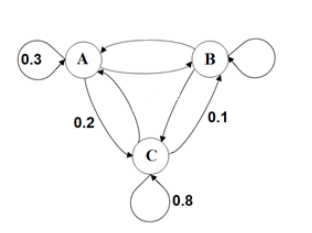
\includegraphics[width=.7\textwidth]{Markov_incomplete.png}
\end{figure}

	\[ 
		\mathbf{P} =
		\begin{bmatrix}
		. & . & 0.2 \\
		0.1 & . & 0.3 \\
		. & . & .
		\end{bmatrix}
	\]

\begin{solution}
        Le diagramme de Markov correspondant est le suivant:

	\begin{figure}[h!]
	    \centering
	    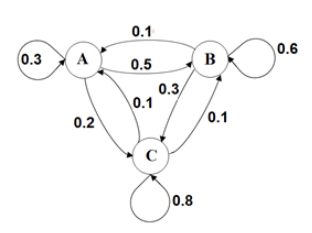
\includegraphics[width=.7\textwidth]{Markov_complete.png}

	\end{figure}
	
	Et sa matrice de transition est:

	\[ 
		\mathbf{P} =
		\begin{bmatrix}
		0.3 & 0.5 & 0.2 \\
		0.1 & 0.6 & 0.3 \\
		0.1 & 0.1 & 0.8
		\end{bmatrix}
	\]
	
    \end{solution}
\end{Exercice}

\begin{Exercice}[10 minutes]\textbf{Problème - Chaîne de Markov}

Suite à  de longs mois d’observation, on a réussi à créer un modèle de prédiction météo en prenant en compte le temps du jour précédent. On sait que lorsqu’il fait beau, les chances qu’il fasse beau le lendemain sont de 80\%, celles qu’il pleuve de 19\% et celles qu’il neige de 1\%. Quand il pleut, les chances qu’il fasse beau le lendemain sont de 20\%, celles qu’il pleuve de 70\% et celles qu’il neige de 10\%. Enfin, quand il neige, les chances qu’il fasse beau le lendemain sont de 10\%, celles qu’il pleuve de 20\% et celles qu’il neige de 70\%.\\
Avec ces informations, dessinez une représentation de Markov sous forme de graphe puis créez la matrice de transition correspondante.


    \begin{solution}
        Le diagramme de Markov correspondant est le suivant:

	\begin{figure}[h!]
	    \centering
	    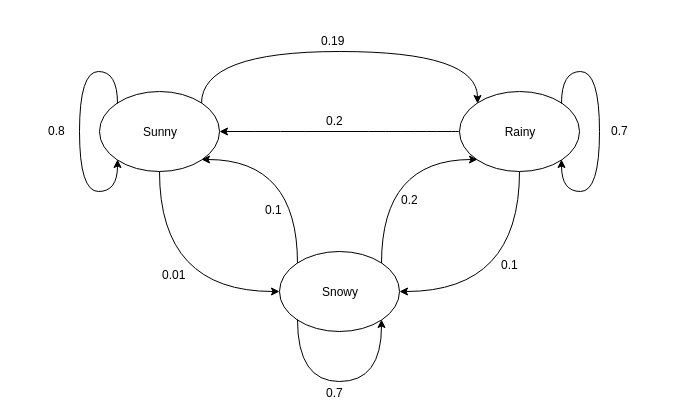
\includegraphics[width=.7\textwidth]{Etats_markov.png}

	\end{figure}
	
	Et sa matrice de transition est:

	\[ 
		\mathbf{P} =
		\begin{bmatrix}
		0.8 & 0.19 & 0.01 \\
		0.2 & 0.7 & 0.1 \\
		0.1 & 0.2 & 0.7
		\end{bmatrix}
	\]
	
    \end{solution}


\end{Exercice}


\begin{Exercice}[10 minutes]\textbf{Le dé - Chaîne de Markov \optionnel}

Un jouer lance un dé à 6 faces un nombre indéterminé de fois. Chaque chiffre à la même probabilité de sortir à chaque lancer. Tant que le joueur n'a pas obtenu tous les chiffres, il continue à lancer le dé. En assimilant la somme des chiffres obtenus aux états d'une chaine de Markov, représentez sa matrice de transition associée.

	 \begin{solution}

	\[ 
		\mathbf{P} =
		\begin{bmatrix}
		0 & 1 & 0 & 0 & 0 & 0 & 0  \\
		0 & 1/6 & 5/6 & 0 & 0 & 0 & 0  \\
		0 & 0 & 2/6 & 4/6 & 0 & 0 & 0  \\
		0 & 0 & 0 & 3/6 & 3/6 & 0 & 0  \\
		0 & 0 & 0 & 0 & 4/6 & 2/6 & 0  \\
		0 & 0 & 0 & 0 & 0 & 5/6 & 1/6  \\
		0 & 0 & 0 & 0 & 0 & 0 & 1 
		\end{bmatrix}
	\]
	 \end{solution}
\end{Exercice}
